\chapter{Implementation}

\section{Data Cleaning and Preprocessing}

As my Data Analysis professor always said, “you can't do much with a dirty, disturbed, and noisy dataset.”  
In fact, I started the implementation with a preliminary phase of \textbf{quality control, cleaning, and normalization of the data}, which is essential for clustering and training the generative model.  
All measurements exported from InfluxDB in CSV format underwent the same processing flow to ensure uniform treatment of energy signals and facilitate the identification of any anomalies or inconsistencies in the raw data~\cite{han2011data, aggarwal2015data}.

\subsection{Quality Check (QC) Audit}

As a first step, I implemented an automated \emph{audit} function, applied to each CSV file with the aim of verifying the quality of the original data and identifying possible critical issues before the actual cleaning phase.  
This control procedure, performed in batches on all measurements exported from InfluxDB, calculates a set of diagnostic statistics and temporal consistency indicators for each column, thus providing a quantitative overview of the dataset’s status.  
The main checks include:
\begin{itemize}
  \item the percentage of missing values (\emph{NaN \%});
  \item descriptive statistics such as standard deviation, minimum, maximum, and number of unique values (useful for identifying constant or nearly constant columns);
  \item analysis of time gaps between consecutive timestamps, by calculating the median interval and detecting any anomalous jumps~\cite{little2019statistical}.
\end{itemize}

To do this, I wrote the function shown in Listing~\ref{lst:auditcsv}, which automates the entire process on a single CSV file, returning both column statistics and an overall temporal consistency report.

\begin{listing}[H]
\begin{minted}[fontsize=\footnotesize,linenos,breaklines,frame=lines,bgcolor=lightgray!10]{python}
def audit_csv(path: Path):
    """
    Loads and analyzes a CSV file, returning:
    - Clean and temporally sorted DataFrame
    - Descriptive statistics per column
    - Diagnostics on temporal gaps
    """
    df = pd.read_csv(path, low_memory=False)
    df = df.loc[:, ~df.columns.str.contains(r"^Unnamed")]
    df["_time"] = pd.to_datetime(df["_time"], utc=True, errors="coerce")

    # Statistical analysis per column
    info = []
    for c in df.columns:
        if c == "_time": continue
        s = pd.to_numeric(df[c], errors="coerce")
        info.append({
            "column": c,
            "nan_%": round(s.isna().mean()*100, 2),
            "std": float(s.std(skipna=True)),
            "unique_vals": int(s.nunique(dropna=True))
        })

    # Diagnosis of time gaps
    dt = df["_time"].diff().dt.total_seconds()
    gaps = {"median_step_s": dt.median(), "big_gaps_%": (dt > 3*dt.median()).mean()*100}

    return df, pd.DataFrame(info), gaps
\end{minted}
\caption{Preliminary audit function for time series datasets.}
\label{lst:auditcsv}
\end{listing}

After validating the function on individual files, I applied it in batches to all measurements in the InfluxDB \emph{bucket}, allowing me to quickly identify the noisiest or most incomplete measurements.  
An excerpt from the control report obtained for the \emph{M2M} measurement is shown in Table~\ref{tab:qc_m2m}.

\begin{longtable}[H]{| l | c | c | c | c | c |}
\hline
\rowcolor[HTML]{F87C58}\textbf{Column} & \textbf{NaN \%} & \textbf{Std} & \textbf{Min} & \textbf{Max} & \textbf{Unique values} \\
\hline
\texttt{Phase 1 Power} & 0.3 & 5.12 & 12.5 & 67.1 & 1221 \\
\hline
\texttt{Phase 2 Power} & 0.1 & 4.87 & 11.8 & 69.3 & 1243 \\
\hline
\texttt{Phase 3 Power} & 0.0 & 6.04 & 13.1 & 72.4 & 1250 \\
\hline
\caption{Excerpt from the Quality Check report for the \emph{M2M} measurement.}
\label{tab:qc_m2m}
\end{longtable}

\subsection{Data Cleaning and Normalization}
\label{subsec:data-cleaning}

After completing the audit phase, I was able to proceed with the \textbf{data cleaning and normalization} process.  
This phase is crucial, as the quality and reliability of the data directly determine the robustness of subsequent analyses~\cite{little2019statistical, aggarwal2015data}.  
I implemented the \emph{data cleaning} flow in a systematic and reusable way, applying it to all time series exported from InfluxDB.  
The pipeline follows a sequence of operations typical of analyses, adapted to the specificities of my dataset.

\begin{listing}[H]
\begin{minted}[fontsize=\footnotesize,linenos,breaklines,frame=lines,bgcolor=lightgray!10]{python}
def clean_timeseries_df(
    df_raw: pd.DataFrame,
    min_std: float = 1e-3,
    interpolate_limit: int = 3,
    resample_rule: str | None = None,      # e.g. "5T"
    winsorize: bool = True,
    winsor_limits=(0.01, 0.99)
) -> pd.DataFrame:
    df = df_raw.copy()
    df["_time"] = pd.to_datetime(df["_time"], utc=True, errors="coerce")
    df = df.dropna(subset=["_time"]).sort_values("_time").set_index("_time")

    # removal of empty or nearly constant columns
    df = df.apply(pd.to_numeric, errors="coerce")
    df = df.dropna(axis=1, how="all")
    df = df.loc[:, df.std(skipna=True) > min_std]

    # aggregation of time duplicates
    if df.index.has_duplicates:
        df = df.groupby(level=0).mean(numeric_only=True)

    # clipping per column to quantiles (winsorization)
    if winsorize:
        q_low, q_hi = df.quantile(winsor_limits[0]), df.quantile(winsor_limits[1])
        for c in df.columns:
            if q_low[c] < q_hi[c]:
                df[c] = df[c].clip(lower=q_low[c], upper=q_hi[c])

    # interpolation and (optional) resampling
    df = df.interpolate(method="time", limit=interpolate_limit, limit_direction="both")
    if resample_rule:
        df = (df.resample(resample_rule)
                .mean(numeric_only=True)
                .interpolate(limit=interpolate_limit, limit_direction="both"))

    return df.reset_index()
\end{minted}
\caption{Dataset cleaning function: temporal parsing, removal of quasi-constant columns, winsorization, and interpolation.}
\end{listing}

First, I convert all timestamps to UTC datetime format, sorting the rows in chronological order and removing any records without a time reference.  
Next, I transform each column into numerical format, eliminating those that are completely empty or nearly constant, i.e., characterized by a negligible standard deviation or a zero minimum–maximum range.  
In the case of temporal duplicates, I consolidate the corresponding rows by calculating the average of the values, so as to obtain a monotonic and consistent time sequence.  
To mitigate the impact of outliers, I then apply \textbf{winsorization} to each column, limiting extreme values to quantiles $[q_{\ell}, q_{h}]$.  
This technique preserves the statistical structure of the central data while reducing the influence of outliers without eliminating them completely.  
For short-term gaps, I perform \emph{time-based} (linear in time) interpolation up to a maximum of three consecutive samples.  
Finally, the function offers the possibility of performing a fixed-step \textbf{resampling} (e.g., every 5 minutes), so as to standardize the sampling frequency between the different measurements and make the series more comparable~\cite{shumway2017time, box2015time}. Once the cleaning was complete, I proceeded to save the datasets in CSV format, sorting the columns deterministically (starting with \texttt{\_time}) and optimizing file size by \textbf{downcasting to} \texttt{float32}.  
This choice allowed me to significantly reduce disk space while maintaining the accuracy necessary for subsequent analyses~\cite{aggarwal2015data}.

\begin{listing}[H]
\begin{minted}[fontsize=\footnotesize,linenos,breaklines,frame=lines,bgcolor=lightgray!10]{python}
def save_clean(df_clean: pd.DataFrame, out_path: Path):
    cols = ["_time"] + sorted([c for c in df_clean.columns if c != "_time"])
    df_clean = df_clean.loc[:, cols]
    for c in df_clean.columns:
        if c != "_time":
            df_clean[c] = pd.to_numeric(df_clean[c], errors="coerce").astype("float32")
    out_path.parent.mkdir(parents=True, exist_ok=True)
    df_clean.to_csv(out_path, index=False)
    return out_path
\end{minted}
\caption{Function for saving clean datasets with stable sorting and numerical optimization.}
\end{listing}

Thanks to this process, I obtained consistent datasets, free of spurious or redundant columns and more robust with respect to the presence of outliers and time gaps.  
All the files used in the subsequent stages of \emph{exploratory analysis}, \emph{clustering}, and \emph{generative training} derive from these cleaned and normalized CSV files.

% ---------------------------

\section{Exploratory analysis and clustering}

After completing the \emph{data cleaning} phase, I began a systematic process of \textbf{exploratory data analysis} (EDA) with the aim of understanding the statistical structure of the energy variables and identifying the most informative fields to be used in the subsequent generative training phase~\cite{han2011data,bishop2006pattern,hastie2009elements}.  
The analysis started from the \emph{M2M} measurement, chosen as a representative case study as it aggregates the behavior of a complete three-phase system, and was then extended to the main selected \emph{Rack*pduA}.

\subsection{Visualization of the main variables}

To study the temporal trend of the most significant electrical signals, I selected the fields relating to current, voltage, power, and energy, generating an independent graph for each.  
This allowed me to identify long-term trends, daily cycles, and the presence of noise or local anomalies in the data~\cite{box2015time,shumway2017time}.

\begin{listing}[H]
\begin{minted}[fontsize=\footnotesize,breaklines,linenos,frame=lines,bgcolor=lightgray!10]{python}
import matplotlib.pyplot as plt

selected_fields = [
    "L1 Current", "L2 Current", "L3 Current",
    "Phase Voltage L1", "Phase Voltage L2", "Phase Voltage L3",
    "3Phase System Voltage", "Apparent Power L2",
    "3Phase System Frequency", "3Phase System Current",
    "3Phase System Apparent Power", "3Phase System Active Power AVG",
    "3Phase System Active Power", "3Phase System Active Energy"
]

df_sel = df_m[["_time"] + selected_fields].copy()

fig, axs = plt.subplots(len(selected_fields), 1, figsize=(15, 3 * len(selected_fields)))
for i, col in enumerate(selected_fields):
    axs[i].plot(df_sel["_time"], df_sel[col], label=col)
    axs[i].set_title(col); axs[i].set_xlabel("Time"); axs[i].grid(True)
plt.tight_layout(); plt.show()
\end{minted}
\caption{Temporal display of the main electrical variables of the measurement \texttt{M2M}.}
\end{listing}

From inspecting the graphs, I observed a clear cyclical behavior in active and apparent power, consistent with typical HPC system loads. Phase voltages, on the other hand, showed greater local variability, indicating instrumental noise or fluctuations in the power supply network.

\subsection{Correlation between variables}

To quantify the linear relationships between the energy fields, I calculated \textbf{Pearson's correlation matrix} on the main signals of the \emph{M2M} measurement, then extended the same procedure to the other measurements.  
The resulting heat map highlights:
\begin{itemize}
  \item strong correlations between \emph{phase currents} and \emph{active powers} ($r \approx 0.9$–$0.95$);
  \item almost perfect correlations between \emph{phase voltages} ($r \approx 0.99$);
  \item a very weak correlation between the \emph{system frequency} and the other quantities;
  \item a moderate correlation between \emph{active energy} and power, consistent with its cumulative behavior.
\end{itemize}

\begin{listing}[H]
\begin{minted}[fontsize=\footnotesize,breaklines,linenos,frame=lines,bgcolor=lightgray!10]{python}
import seaborn as sns

# Only numeric columns (excluding timestamp)
corr = df_selected.drop(columns="_time").corr()
plt.figure(figsize=(10, 8))
sns.heatmap(corr, annot=True, fmt=".2f", cmap="coolwarm", square=True)
plt.title(f"Correlation between field - {measurement}")
plt.tight_layout()
plt.show()
\end{minted}
\end{listing}

\begin{figure}[H]
\centering
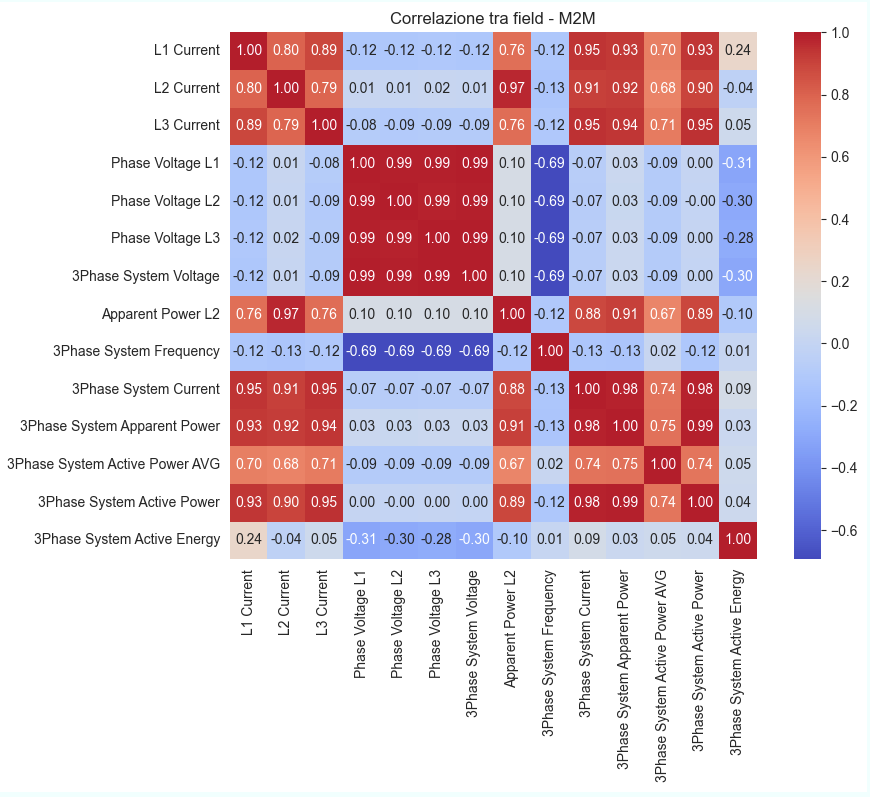
\includegraphics[width=0.85\textwidth]{images/matr_corr.png}
\caption{Correlation matrix between the main electric fields of the \emph{M2M} measurement.}
\label{fig:m2m_heatmap}
\end{figure}

This analysis allowed me to identify groups of highly correlated and redundant variables, providing a solid basis for the subsequent selection of the most representative features to be used in clustering and generation models~\cite{bishop2006pattern,han2011data,hastie2009elements,pearson1895correlation}.

\subsection{Autocorrelation of signals}

I deepened the temporal analysis by focusing on the variable \texttt{3Phase System Active Power AVG}, which summarizes the overall energy behavior of the system.  
I calculated the \textbf{autocorrelation function} (\emph{ACF}) up to 100 delays, highlighting a slow decay and the presence of \textbf{cyclical patterns} attributable to daily and weekly periodicity.

\begin{listing}[H]
\begin{minted}[fontsize=\footnotesize,breaklines,linenos,frame=lines,bgcolor=lightgray!10]{python}
from statsmodels.graphics.tsaplots import plot_acf

plot_acf(df_selected["3Phase System Active Power AVG"].dropna(), lags=100)
plt.title("Autocorrelation - 3Phase System Active Power AVG")
plt.show()
\end{minted}
\end{listing}

\begin{figure}[H]
\centering
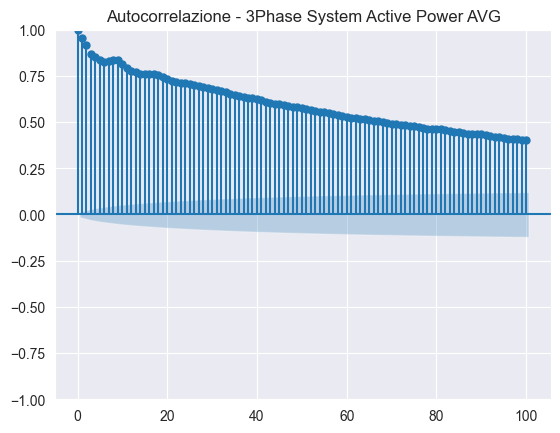
\includegraphics[width=0.7\textwidth]{images/autocorrelation_m2m.png}
\caption{Autocorrelation function (\emph{ACF}) of the average three-phase power (\emph{M2M}) up to 100 delays.}
\label{fig:m2m_autocorr}
\end{figure}

The ACF analysis provided two key insights:
\begin{enumerate}
  \item energy loads in HPC systems are not purely random, but follow regular cycles linked to the use of computational resources~\cite{box2015time,shumway2017time};
  \item the presence of stable periodicity justifies the introduction of \textbf{cyclic features} (sine and cosine of hour, day, and month) in the preprocessing pipeline, making the intrinsic seasonality of the data explicit and improving the model's ability to learn recurring patterns~\cite{bishop2006pattern,hastie2009elements}.
\end{enumerate}

\subsection{Clustering with PCA and \textit{k}-Means}

To identify \textbf{latent structures} within energy signals from HPC systems, I developed a multi-step clustering workflow that integrates statistical analysis, dimensionality reduction, and visual interpretation of data.  
The objective of this phase was twofold: on the one hand, I needed to understand the intrinsic variability of the signals and identify recurring operating regimes; on the other hand, I needed to provide a compact and interpretable representation of the data for the subsequent phases~\cite{bishop2006pattern,hastie2009elements,han2011data,aggarwal2015data}.

\begin{enumerate}
  \item \textbf{Feature extraction.}  
  I divided each signal into time windows of 128 steps (with stride 64) and calculated a set of statistical and dynamic descriptors for each window—mean, standard deviation, RMS energy, mean slope, and lag-1 autocorrelation—for each power channel.  
  This approach allowed me to transform the continuous time series into a structured set of numerical vectors, more suitable for multivariate analysis.

  \item \textbf{Cleaning and scaling.}  
  I subjected the features obtained in this way to a robust normalization process to ensure greater numerical stability and reduce the influence of outliers or annoying measurement noise.  
  In particular, I performed:
  \begin{itemize}
      \item removal of constant or entirely null columns;
      \item imputation of missing values with the median for each feature;
      \item \emph{clipping} at the 1st–99th percentile to attenuate outliers;
      \item the application of a \emph{RobustScaler} (based on quantiles 5–95\%) to obtain a stable and comparable distribution between features.
  \end{itemize}

\begin{listing}[H]
\begin{minted}[fontsize=\footnotesize,breaklines,linenos,frame=lines,bgcolor=lightgray!10]{python}
from sklearn.preprocessing import RobustScaler
import numpy as np

F = Feat_tr.astype("float64")
F[~np.isfinite(F)] = np.nan
col_med = np.nanmedian(F, axis=0)
inds = np.where(np.isnan(F))
if inds[0].size: F[inds] = np.take(col_med, inds[1])
var = np.var(F, axis=0)
F = F[:, var > 1e-12]                # removes quasi-constants
lo, hi = np.quantile(F, [0.01, 0.99], axis=0)
F = np.clip(F, lo, hi)               # clipping outliers
Fz = RobustScaler().fit_transform(F) # robust scaling
\end{minted}
\end{listing}

  \item \textbf{Dimensional reduction (PCA).}  
  To analyze the internal structure of the features, I applied \emph{Principal Component Analysis} (PCA), reducing the variable space to:
  \begin{itemize}
      \item 2 principal components for graphical visualization (\emph{PCA-2D});
      \item up to 10 components for the actual input to clustering (\emph{PCA-10D}).
  \end{itemize}
  This transformation allowed me to capture over 80\% of the total variance, thus preserving essential information at a reduced computational cost~\cite{jolliffe2002pca}.

  \item \textbf{k-Means and optimal selection of $k$.}  
  I then applied the \emph{k-Means} algorithm for values of $k$ between 2 and 6, evaluating the quality of each configuration using the \emph{silhouette score}, a measure of internal cohesion and separation between clusters~\cite{rousseeuw1987silhouettes}.
\end{enumerate}

\subsubsection{Evaluation and results}

Analysis of the \emph{silhouette score} values (Figure~\ref{fig:silhouette}) showed a maximum for $k=5$ ($s \approx 0.42$), indicating a clear separation between the groups and a well-defined latent structure in the data.  
The two-dimensional projections obtained with PCA show distinct and consistent clusters, interpretable as different \textbf{operating regimes} of the HPC system and its power supply subsystem.

\begin{figure}[H]
\centering
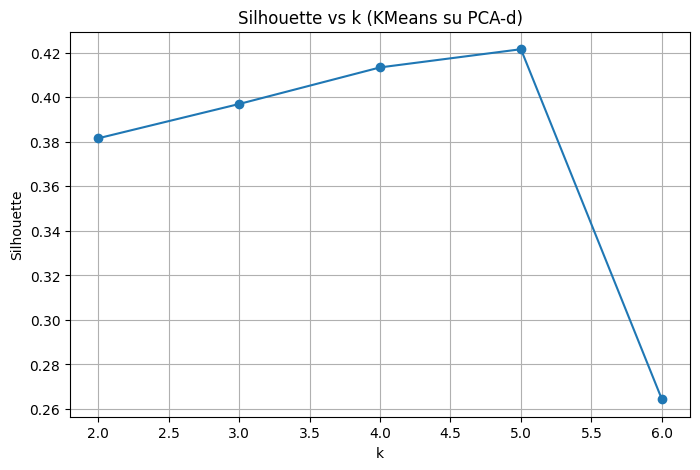
\includegraphics[width=0.50\textwidth]{images/silhouette_plot.png}
\caption{\emph{Silhouette score} trend as $k$ varies.}
\label{fig:silhouette}
\end{figure}

\begin{figure}[H]
\centering
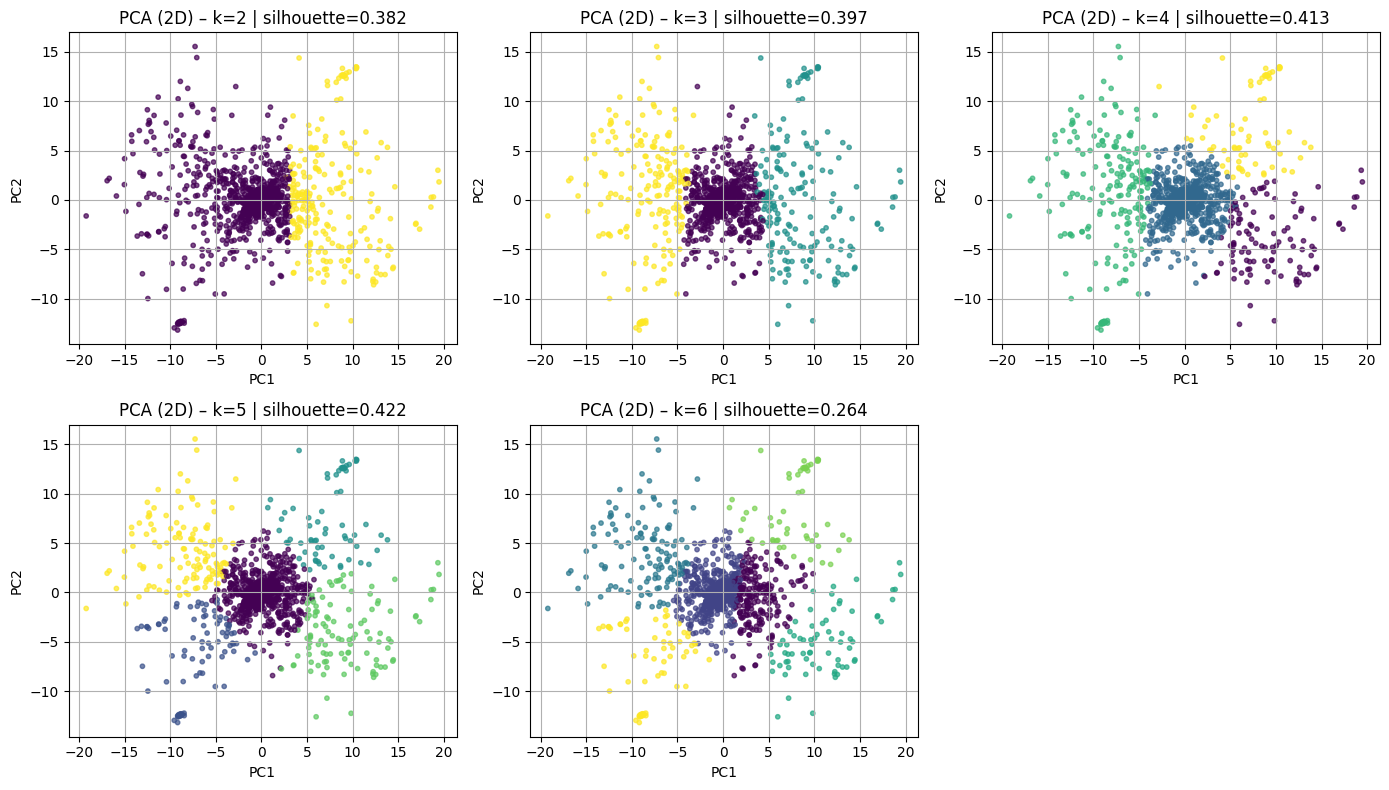
\includegraphics[width=0.70\textwidth]{images/pca2d_all_k.png}
\caption{PCA-2D projections of clusters obtained with $k = 2 \dots 6$.  
A progressive refinement of the separation can be observed up to $k=5$, beyond which the clusters begin to fragment.}
\label{fig:pca2d_all_k}
\end{figure}

\begin{figure}[H]
\centering
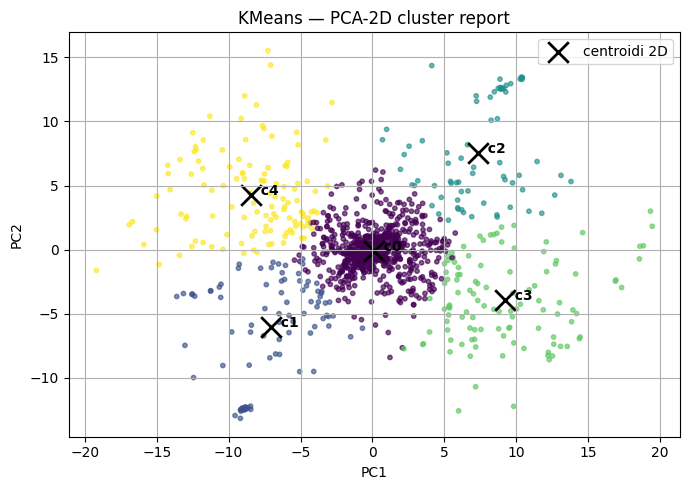
\includegraphics[width=0.50\textwidth]{images/pca2d_cluster_report.png}
\caption{Distribution of data in PCA-2D space with labeled centroids for each cluster ($k=5$).  
There is a clear separation between the density regions, corresponding to different energy regimes.}
\label{fig:pca2d_cluster_report}
\end{figure}

\subsubsection{Interpretation of clusters}

As I mentioned, analysis of the results allowed me to identify three main categories of behavior:
\begin{itemize}
  \item \textbf{Stable clusters}, characterized by almost constant signals and associated with basic loads or periods of system inactivity;
  \item \textbf{Dynamic clusters}, with rapid variations and power peaks, typical of periods of intense computing;
  \item \textbf{Intermediate clusters}, interpretable as transitional states or partial activity between the two extremes.
\end{itemize}

These partitions provide a clear representation of \textbf{recurring energy patterns} in the racks and form an empirical basis for the subsequent \textbf{conditional generation of synthetic series} using diffusion models such as \emph{WaveStitch}.

% ----------------------

\section{Training, scenario imputation, and conditional generation with WaveStitch}

After completing the steps described so far, I finally started the \textbf{training and conditional generation} phase with the \emph{WaveStitch} model.  
This part of the work represents the experimental core of my project, with the interesting aim of: on the one hand, evaluating the model's ability to adapt to real data affected by noise and irregularities; on the other hand, verifying the possibility of producing \textbf{plausible synthetic scenarios}, useful for simulation, testing, and much more.

\subsection{Model training}

I began training with the \emph{M2M} metric, selected for its regularity and its ability to represent, as I mentioned earlier, the overall energy performance of the HPC system.  
The configuration adopted for training was defined in order to balance complexity, stability, and generalization capacity, with the following main hyperparameters:

\begin{itemize}
  \item \textbf{Backbone}: \texttt{S4}, chosen for its efficiency in modeling long sequences using structured memory;
  \item \textbf{Window size}: 96, to capture a broader and more informative temporal context;
  \item \textbf{Stride}: 8, to ensure high overlap and improve continuity between successive windows;
  \item \textbf{Epochs}: 100, ensuring stable convergence of the learning process;
  \item \textbf{Batch size}: 64, balancing numerical stability and memory limitations;
  \item \textbf{Diffusion timesteps}: 200, higher than those in the original paper to handle the greater variability of HPC signals;
  \item \textbf{Cyclic features}: \texttt{month, day, hour}, useful for capturing daily and seasonal periodicity.
\end{itemize}

To ensure flexibility in experimentation, I created a parametric Python script that dynamically constructs the execution command of the \texttt{training\_wavestitch.py} file, allowing training sessions to be started in a controlled manner on different datasets and with variable configurations~\cite{gu2021s4}.

\begin{listing}[H]
\begin{minted}[fontsize=\footnotesize,breaklines,linenos,frame=lines,bgcolor=lightgray!10]{python}
cmd = [
    sys.executable, "training_wavestitch.py",
    "-dataset", DATASET,
    "-backbone", BACKBONE,
    "-window_size", str(WINDOW_SNE),
    "-stride", str(STRIDE),
    "-epochs", str(EPOCHS),
    "-batch_size", str(BATCH_SNE),
    "-hdim", str(HDIM),
    "-layers", str(LAYERS),
    "-timesteps", str(TIMESTEPS),
    "-s4_dropout", str(S4_DROPOUT),
    "-propCycEnc", PROP_CYC,
]
res = subprocess.run(cmd, text=True, capture_output=True)
print(res.stdout)
\end{minted}
\end{listing}

The resulting model is saved in an \textbf{enriched checkpoint}, which not only contains the weights of the neural network, but also includes: the complete configuration of the training hyperparameters, the ordered list of the dataset columns, the indication of cyclic and non-cyclic features, and the actual input and output dimensions.  
The final checkpoint was named \texttt{model\_prop.pth}, indicating the presence of cyclic features (\emph{propCycEnc}) in the training.

\begin{figure}[H]
\centering
\begin{tikzpicture}[
    font=\footnotesize\sffamily,
    node distance=1.8cm,
    process/.style={
        rectangle, rounded corners,
        draw=black, very thick,
        text centered,
        minimum width=4.2cm,
        minimum height=1.1cm,
        align=center
    },
    arrow/.style={thick,->,>=stealth}
]
\node[process, fill=cyan!15] (prep) {Preprocessing\\\textit{(scaling, encoding)}};
\node[process, fill=teal!15,  below=of prep] (win) {Windowing\\\textit{(windowing, stride)}};
\node[process, fill=lime!15,  below=of win]  (train) {Training\\\textit{(denoising)}};
\node[process, fill=gray!15,  below=of train] (ckpt) {Checkpoint\\\textit{rich (.pth)}};

\draw[arrow] (prep) -- (win);
\draw[arrow] (win)  -- (train);
\draw[arrow] (train) -- (ckpt);

\node[right=0.7cm of prep]  {\texttt{df\_cleaned}};
\node[right=0.7cm of win]   {\textit{window size = 96, stride = 8}};
\node[right=0.7cm of train] {\textit{loss MSE, 100 epochs}};
\node[right=0.7cm of ckpt]  {\texttt{model\_prop.pth}};
\end{tikzpicture}
\caption{Simplified diagram of the training phase: preprocessing $\rightarrow$ windowing $\rightarrow$ denoising $\rightarrow$ rich checkpoint.}
\label{fig:training_pipeline}
\end{figure}

This configuration produced \textbf{stable convergence} on the \emph{M2M} data, with a progressive reduction in loss and final values comparable to those reported in the original work~\cite{wavestitch,ho2020ddpm,dhariwal2021improved}.  
Doing the same with the racks, I can say that the result demonstrated how effectively \emph{WaveStitch} can adapt to real datasets, which are noisier and more complex than the original benchmarks, confirming its robustness and generalization capabilities.

\subsection{Conditional synthetic generation}

After completing the training phase, I started the \textbf{conditional synthetic generation} using the previously trained \emph{rich checkpoint}, without the need for retraining.  
The procedure was managed using the script:\\
\texttt{synthesis\_wavestitch\_pipeline\_strided\_preconditioning.py},  
which automatically reads the hyperparameters from the checkpoint and realigns all key parameters — \emph{backbone}, window, stride, and number of \texttt{timesteps} — ensuring perfect consistency between the training and generation phases~\cite{wavestitch,ho2020ddpm,dhariwal2021improved}.  
To explore different temporal granularities of imputation, I defined three distinct scenarios: \textbf{F (Fine)} — point imputation, suitable for local \emph{forecasting}; \textbf{C (Coarse)} — reconstruction of extended time blocks or those with significant gaps; \textbf{M (Mid)} — intermediate scenario, useful for modeling transitions or progressive variations.

In order to improve the multivariate fidelity and temporal continuity of the generated sequences, I introduced two fundamental extensions: a \textbf{configurable stitching loss} in the overlap areas between parallel windows, based on \texttt{mse}, \texttt{mae}, or shape-based metrics (\texttt{cosine}, \texttt{pearson})~\cite{dhariwal2021improved,ho2020ddpm}; a \textbf{correlation regularization between channels} (\(\lambda_{\text{corr}} = 0.30\), \texttt{pearson} metric), to preserve the statistical relationships between connected variables such as currents and powers~\cite{bishop2006pattern,hastie2009elements}.


\begin{listing}[H]
\begin{minted}[fontsize=\footnotesize,breaklines,linenos,frame=lines,bgcolor=lightgray!10]{python}
# Synthesis consistent with checkpoint, three masks: F / C / M
for mask in MASKS:
    out_dir_mask = os.path.join(BASE_OUT, mask)
    os.makedirs(out_dir_mask, exist_ok=True)

    cmd = [
        sys.executable, SYNTH_SCRIPT,
        "-dataset", DATASET,
        "-backbone", BACKBONE,
        "-window_size", str(WINDOW_SIZE),
        "-stride", str(STRIDE),
        "-timesteps", str(TIMESTEPS),
        "-hdim", str(HDIM),
        "-layers", str(LAYERS),
        "-batch_size", str(BATCH_SIZE_SYNTH),
        "-synth_mask", mask,
        "-n_trials", "1",
        "-propCycEnc", PROP_CYC,
        "-s4_lmax", str(S4_LMAX),
        "-s4_dstate", str(S4_DSTATE),
        "-s4_dropout", str(S4_DROPOUT),
        "-s4_layernorm", str(S4_LAYERNORM),
        "-ckpt", CKPT,
        "-lambda_corr", str(LAMBDA_CORR),
        "-corr_mode", CORR_MODE,
        "-out_dir", out_dir_mask,
    ]

    print("[CMD] " + " ".join(shlex.quote(c) for c in cmd))
    res = subprocess.run(cmd, text=True, capture_output=True)
# (repeat with -synth_mask C and M)
\end{minted}
\caption{Conditional synthesis pipeline with automatic checkpoint alignment and multiscenario generation.}
\end{listing}

Each run generates two separate files: \texttt{real.csv}, containing the actual reference segment, and \texttt{synth*.csv}, representing the synthetic output produced by the model.

\subsection{Preliminary observations}

The first experiments conducted on my datasets showed that \emph{WaveStitch}, even in the presence of noise and outliers, is able to generate sequences \textbf{that are statistically consistent} with the overall properties of the real data.  
Looking at the point-by-point comparison, I noticed that the synthetic data tends to smooth out the most extreme peaks, producing more regular and realistic curves.  
This behavior, while reducing the local linear correlation with the original series, actually confirms the model’s remarkable ability to \textbf{generalize plausible behaviors} instead of rigidly replicating the outliers present in the source data.  

Throughout this process, I was able to observe the excellent \textbf{computational scalability} of the model.  
Thanks to the \emph{parallel generation mechanism with stitching}, the synthesis proved to be very fast, in line with the results of the original work.  
The ability to dynamically adjust the \emph{stitching} and \emph{correlation regularization} components made the pipeline flexible and adaptable to multiple experimental scenarios, ranging from short-term \emph{forecasting} to the imputation of missing time blocks.

\subsection{Extension to other HPC datasets}

As I mentioned, I replicated the entire training and synthesis process on individual rack measurements, which are characterized by greater noise and temporal irregularities.  
This systematic comparison between aggregated and local datasets allowed me to confirm that \textbf{the quality and regularity of the input signal directly influence the stability and statistical fidelity of the synthetic generation}.  
The quantitative results (MAE, RMSE, MAPE, Pearson correlation) and qualitative analyses (visual analysis, autocorrelations, and cross-correlations) will be explored in more detail in the following chapters, where I will show how \emph{WaveStitch} consistently reproduces both the average trends and the temporal structure of HPC energy signals.
% -----------------------------

\subsection{Imputation of missing values with WaveStitch}

The most valuable part of my work consists of the following three phases.  
I started by imputing missing values, which represented the most direct test of \textbf{conditional generation} based on \emph{WaveStitch}.  
The goal is to estimate the missing values $y^{\star}(t)$ at unobserved times $\mathcal{M}$, starting from a real series $y(t)$ and the synthetic trajectory $\tilde{y}(t)$ produced by the model~\cite{box2015time,shumway2017time}:
\[
y^{\star}(t) \approx \tilde{y}(t) \quad \text{for } t \in \mathcal{M}.
\]

In the event that the \texttt{real.csv} file does not contain null values, I introduced an artificial mask with amplitude $|\mathcal{M}| = 100$, so that I could quantitatively evaluate the quality of the imputation with respect to the original \emph{ground truth}~\cite{little2019statistical}.  
In this way, I was able to accurately quantify the effectiveness of the model even in the absence of truly missing data.

\begin{figure}[H]
\centering
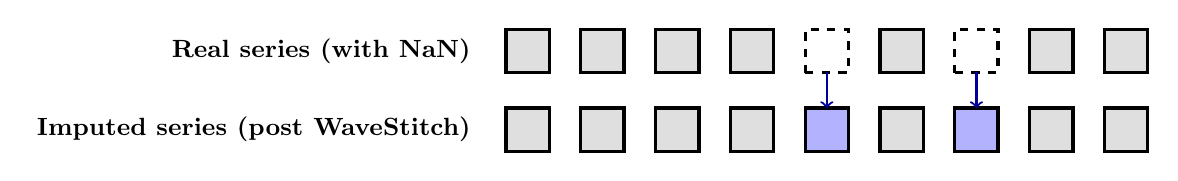
\begin{tikzpicture}[
    every node/.style={font=\small},
    real/.style={draw, very thick, fill=gray!25, minimum height=0.55cm, minimum width=0.55cm},
    nan/.style={draw, very thick, fill=white, dashed, minimum height=0.55cm, minimum width=0.55cm},
    imputed/.style={draw, very thick, fill=blue!30, minimum height=0.55cm, minimum width=0.55cm}
]
\def\N{9}\def\xStart{0.8}\def\dx{0.95}\def\yReal{0.8}\def\yImpu{-0.2}
\def\nanA{4}\def\nanB{6}

\node[anchor=east] at (0.2,\yReal) {\textbf{Real series (with NaN)}};
\node[anchor=east] at (0.2,\yImpu) {\textbf{Imputed series (post WaveStitch)}};

\foreach \k in {0,...,\numexpr\N-1\relax} {
  \pgfmathsetmacro\x{\xStart + \k*\dx}
  \ifnum\k=\nanA \node[nan] at (\x,\yReal) {}; 
  \else\ifnum\k=\nanB \node[nan] at (\x,\yReal) {}; 
  \else \node[real] at (\x,\yReal) {}; 
  \fi\fi
  
  \ifnum\k=\nanA \node[imputed] at (\x,\yImpu) {}; 
  \else\ifnum\k=\nanB \node[imputed] at (\x,\yImpu) {}; 
  \else \node[real] at (\x,\yImpu) {}; 
  \fi\fi
}

\pgfmathsetmacro{\xa}{\xStart + \nanA*\dx}
\pgfmathsetmacro{\xb}{\xStart + \nanB*\dx}
\draw[->, thick, blue!60!black] (\xa,\yReal-0.27) -- (\xa,\yImpu+0.27);
\draw[->, thick, blue!60!black] (\xb,\yReal-0.27) -- (\xb,\yImpu+0.27);

\end{tikzpicture}
\caption{Conceptual diagram of imputation: NaNs (white, dashed) are replaced by imputed values (blue) generated by WaveStitch.}
\label{fig:imputation_schema}
\end{figure}

\paragraph{Alignment and selection of the target column.}
Since the \texttt{real.csv} and \texttt{synth*.csv} files may have slightly misaligned timestamps, I implemented a \textbf{merge-as-of} alignment, based on a nearest-neighbor match on times~\cite{han2011data}.  
This choice ensures robustness even in the presence of minimal sampling differences.  
The column of interest $v$ is identified through a hierarchical selection procedure:  
if the user provides an explicit \texttt{value\_col} parameter, I use that;  
otherwise, the function automatically attempts to detect common columns (e.g., \texttt{3Phase System Active Power AVG});  
as a last fallback, it chooses the first numeric column shared between real and synthetic files — avoiding common mistakes such as accidentally selecting the timestamp column as the target variable.

\paragraph{Affine calibration and clipping.}
To compensate for possible differences in scale or offset between real and synthetic data, I introduced an \textbf{affine calibration}:
\[
\hat{y}_{\text{synth}}(t) = a \cdot y_{\text{synth}}(t) + b,
\]
with $(a,b)$ estimated via linear regression on the observed points $t \in \mathcal{O}$~\cite{han2011data}.  
I considered two operating modes:
\begin{itemize}
  \item \textbf{Global}, which estimates $(a,b)$ across the entire series — more stable but less sensitive to regime changes;
  \item \textbf{Local}, which estimates $(a_\ell,b_\ell)$ for each contiguous block of NaN within a window $\pm W$, more suitable for non-stationary or drifting signals.
\end{itemize}

Finally, I applied a \textbf{quantile clipping} on $[q_\ell,q_h] = [0.01,0.99]$, anchoring the scale to the real signal support and reducing the impact of outliers and heavy tails~\cite{little2019statistical,aggarwal2015data}.

\paragraph{Filling strategy.}
The imputation process consists of four steps:
\begin{enumerate}
  \item optional generation of artificial NaNs (for quantitative evaluation);
  \item estimation of affine parameters $(a,b)$ or $(a_\ell,b_\ell)$ on observed points only;
  \item reconstruction of missing values through affine transformation:
  \[
  y^\star(t) =
  \begin{cases}
  a_\ell\,y_{\text{synth}}(t)+b_\ell, & \text{if \texttt{calibrate=local}}, \\[2pt]
  a\,y_{\text{synth}}(t)+b, & \text{otherwise;}
  \end{cases}
  \]
  \item \emph{tapering at the edges}, i.e., a linear blending on $\pm$ \texttt{half\_window} to eliminate discontinuities at the hole boundaries~\cite{shumway2017time}.
\end{enumerate}

\paragraph{Control parameters and robustness.}
I clearly designed the function to be adaptable to different inputs and distinct datasets.  
Thanks to this configuration, the function proved to be robust on heterogeneous data, able to automatically handle differences in sampling, scaling, and naming without manual intervention.

\begin{listing}[H]
\begin{minted}[fontsize=\footnotesize,breaklines,linenos,frame=lines,bgcolor=lightgray!10]{python}
# WaveStitch-guided imputation with calibration and clipping
csv_path, metrics = impute_missing_with_wavestitch(
    dataset="M2M", mask="M",
    base_path="notebooks/generated",
    value_col=None,          # automatic selection of target column
    n_missing=100,           # artificial mask for quantitative evaluation
    calibrate="local",       # calibration for NaN blocks
    local_window=100,        # window width ±W
    clip_quantiles=(0.01,0.99)  # clipping for energy outliers
)
print(metrics)  # -> MAE / RMSE / Corr on masked positions
\end{minted}
\caption{Example of imputation with WaveStitch and quantitative evaluation.}
\label{lst:wavestitch_imputation}
\end{listing}

I achieved an excellent compromise between fidelity and numerical stability simply by combining \texttt{calibrate=local} and \texttt{clip\_quantiles=(0.01,0.99)}, maintaining consistency even on noisy signals or those affected by outliers~\cite{little2019statistical,shumway2017time}.

\paragraph{Empirical observations.}
In tests conducted on \emph{M2M} (mask M), the \textbf{global calibration} produced regular and conservative estimates, while the \textbf{local calibration} significantly improved the reconstruction of long gaps and transitions between different regimes.  
The \textbf{clipping} reduced the effect of extreme values, improving the MAE and RMSE metrics, while the \textbf{tapering} eliminated visual discontinuities at the edges of the imputed segments.  
Overall, the results show a solid balance between statistical fidelity and signal regularity, with average correlation values $r > 0.9$ on artificial masks, as I will show in the next chapter.

% -------------------------

\subsection{Simulation of scenarios via STL decomposition}

To explore hypothetical \emph{what--if} scenarios on the energy consumption profiles of HPC systems, I implemented a simulation procedure based on the \textbf{STL seasonal decomposition} (\emph{Seasonal-Trend decomposition using Loess}).  
The goal was to understand how the different components—trend, seasonality, and residual—contribute to the overall shape of the signals, and how their modulation could simulate operational variations, drifts, or local shocks.  
Formally, the real series $y(t)$ is decomposed into three main components:
\[
y(t) = T(t) + S(t) + R(t),
\]
where $T(t)$ represents the long-term trend, $S(t)$ the seasonal cyclic component, and $R(t)$ the unstructured residual.  
Starting from this decomposition, I introduced three scaling factors $(\alpha, \beta, \gamma)$ and a local shock term $\Delta$ to construct new synthetic scenarios:
\[
y_{\text{scen}}(t) = \beta \, T(t) + \alpha \, S(t) + \gamma \, R(t) + \mathbf{1}_{\{t=t^\star\}} \cdot \Delta.
\]
This formulation makes it possible to amplify or attenuate seasonality, modify long-term trends, control residual noise, and introduce controlled impulse peaks—for example, to simulate sudden load events or temporary failures.

\paragraph{Conceptual diagram.}
\begin{figure}[H]
\centering
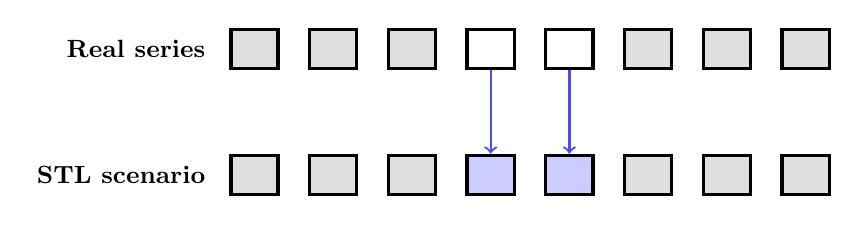
\begin{tikzpicture}[
    every node/.style={font=\small},
    rect/.style={draw, very thick, minimum width=0.6cm, minimum height=0.5cm},
    arrow/.style={thick,->,>=stealth}
]
% Real series
\node[anchor=east] at (-0.5,1.0) {\textbf{Real series}};
\foreach \x in {0,1,...,7}{
    \node[rect, fill=gray!25] (r\x) at (\x,1) {};
}
\node[rect, fill=white] (r3) at (3,1) {};
\node[rect, fill=white] (r4) at (4,1) {};

% STL scenario
\node[anchor=east] at (-0.5,-0.6) {\textbf{STL scenario}};
\foreach \x in {0,1,...,7}{
    \node[rect, fill=gray!25] (s\x) at (\x,-0.6) {};
}
\node[rect, fill=blue!20] (s3) at (3,-0.6) {};
\node[rect, fill=blue!20] (s4) at (4,-0.6) {};

% Arrows
\draw[->, thick, blue!70] (r3.south) -- (s3.north);
\draw[->, thick, blue!70] (r4.south) -- (s4.north);
\end{tikzpicture}
\caption{Conceptual diagram of STL simulation: modified values (white) are replaced with generated values (blue) after seasonal adjustment or the introduction of a local shock~\cite{shumway2017time, cleveland1990stl}.}
\label{fig:stl_schema_concettuale}
\end{figure}

\paragraph{Automatic column detection.}
Since the generated CSV files may contain heterogeneous structures, I made the \texttt{simulate\_scenario\_stl\_flex} function fully autonomous in identifying key columns.  
In particular, the function automatically detects:
\begin{enumerate}
  \item the time column, through a heuristic search among common names (\texttt{date}, \texttt{time}, \texttt{timestamp});
  \item the target value column, chosen from a list of known names or, if none are found, the first valid numeric column.
\end{enumerate}

\paragraph{Determination of the seasonal period.}
The quality of the STL decomposition depends strongly on the correct estimation of the period $P$, i.e., the number of samples that constitute a complete cycle.  
To determine $P$, I developed a robust inference strategy based on timestamps: estimating the median interval $\Delta t$ between two observations and setting
\[
P \approx \left\lfloor \frac{86400}{\Delta t} \right\rfloor,
\]
which corresponds to the average number of daily samples (e.g., $P \approx 288$ for 5-minute data, or $P \approx 24$ for hourly data).  
When the series is too short to observe multiple complete cycles, the period is reduced to $\max(2, \lfloor |y|/3 \rfloor)$ to ensure numerical stability.  
Nevertheless, I left the option to manually specify $P$ in case of prior knowledge.

\paragraph{Implementation and main parameters.}
The simulation function accepts flexible parameters to modulate the three components:
\begin{itemize}
  \item \texttt{season\_scale} $(\alpha)$ — scale of the seasonal component $S(t)$ (default 1.2);
  \item \texttt{trend\_scale} $(\beta)$ — trend amplification factor for $T(t)$ (default 1.0);
  \item \texttt{resid\_scale} $(\gamma)$ — control for residual noise $R(t)$ (default 1.0);
  \item \texttt{shock\_idx}, \texttt{shock\_mag} — time index and amplitude of a possible impulsive shock $\Delta$;
  \item \texttt{period} — STL period, calculated automatically or defined by the user.
\end{itemize}
The result is a CSV file with an additional column \texttt{\{value\_col\}\_scenario} and a preview graph showing the first 600 samples.

\paragraph{Application to the \texttt{M2M} dataset.}
I applied this procedure to the \texttt{M2M} dataset (5-minute sampling, $P = 288$) considering two scenario configurations:
\begin{enumerate}
  \item 20\% amplification of the seasonal component without shock;
  \item 30\% amplification of the seasonal component with the addition of a local shock.
\end{enumerate}

\begin{listing}[H]
\begin{minted}[fontsize=\footnotesize,breaklines,linenos,frame=lines,bgcolor=lightgray!10]{python}
# STL scenario simulation on M2M
base = "notebooks/generated"

csv_out, png_out = simulate_scenario_stl_flex(
    dataset="M2M", mask="M", base_path=base,
    value_col="3Phase System Active Power AVG",
    season_scale=1.2, trend_scale=1.0, resid_scale=1.0,
    period=288, shock_idx=None, shock_mag=0.0
)

# Variant with amplified seasonality and local shock
csv_out2, png_out2 = simulate_scenario_stl_flex(
    dataset="M2M", mask="M", base_path=base,
    value_col="3Phase System Active Power AVG",
    season_scale=1.3, trend_scale=1.0, resid_scale=1.0,
    period=288, shock_idx=10000, shock_mag=500.0
)
\end{minted}
\caption{Running the STL simulation on \texttt{M2M}: seasonal amplification and optional shock.}
\label{lst:scenario_stl_launch}
\end{listing}

Both scenarios keep $T(t)$ and $R(t)$ unchanged, allowing the impact of the periodic component alone to be isolated and analyzed.  
The progressive increase of $\alpha$ accentuates daily cyclicality without distorting the underlying trend.  
The scenario with 30\% amplified seasonality shows more reactive behavior to daily peaks, which is useful for testing the robustness of forecasting models and overall energy stability~\cite{box2015time,shumway2017time, cleveland1990stl}.

\paragraph{Limitations and interpretation.}
The STL decomposition assumes an additive structure and quasi-stationary seasonality; in the presence of regime shifts or multiplicative effects, linear scaling may over- or underestimate the true impact~\cite{cleveland1990stl,shumway2017time}.  
In such contexts, the simulated outputs should be interpreted as \textbf{qualitative what--if analyses}, useful for stress testing and strategic planning rather than for accurate point forecasting.  
Integration with conditional generation through \emph{WaveStitch}, on the other hand, enables the creation of consistent multivariate synthetic scenarios, preserving both temporal and inter-variable dependencies observed in real data—and it has been extremely satisfying to verify this in practice.

% ------------------------

\section{Conditional forecasting with WaveStitch}
\label{sec:forecasting-wavestitch}

Here we are at the third and, for me, most interesting phase. In this section, I describe the \emph{forecasting} module that I developed following the conditional generation with \emph{WaveStitch}.  
The goal was to evaluate the model’s ability to project the local dynamics of a time series toward a short-term future horizon, maintaining consistency in both scale and shape with respect to the actual data.  
My operational idea was very straightforward: once the synthetic sequence was aligned with the real series (\texttt{real.csv} and \texttt{synth*.csv}), I extracted the tail of length $h$ (the \emph{horizon}) and used it as the predictive base for the next steps.  
To compensate for possible level or scale misalignments between real and synthetic data, I applied an \textbf{affine calibration} on the observed tail, estimating the parameters $(a,b)$ by linear regression on the common endpoints:
\[
y_{\text{real}} \approx a\,y_{\text{synth}} + b,
\quad\text{with}\quad
(a,b) = \arg\min_{a,b} \| y_{\text{tail}} - (a\,x_{\text{tail}} + b) \|_2^2,
\]
possibly including ridge regularization to handle noise or high variance.  
The final forecast is then obtained by applying the same transformation to the subsequent $h$ synthetic points~\cite{bishop2006pattern,hastie2009elements}:
\[
\widehat{y}_{t+1:t+h} = a\,y^{\text{synth}}_{t+1:t+h} + b.
\]

\begin{figure}[H]
\centering
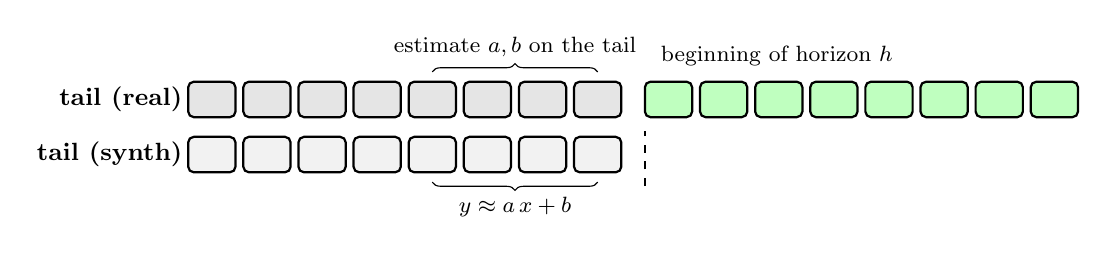
\begin{tikzpicture}[
  every node/.style={font=\small},
  box/.style={draw, thick, minimum width=0.6cm, minimum height=0.45cm, rounded corners=2pt, fill=gray!20},
  synth/.style={draw, thick, minimum width=0.6cm, minimum height=0.45cm, rounded corners=2pt, fill=gray!10},
  forecast/.style={draw, thick, minimum width=0.6cm, minimum height=0.45cm, rounded corners=2pt, fill=green!25}
]

\def\yreal{0.9}
\def\ysynth{0.2}
\def\xmin{0.3}
\def\xstep{0.7}

\node[anchor=east] at (\xmin-0.25,\yreal) {\textbf{tail (real)}};
\node[anchor=east] at (\xmin-0.25,\ysynth) {\textbf{tail (synth)}};

\foreach \i in {0,...,7} {
  \pgfmathsetmacro\x{\xmin + \i*\xstep}
  \node[box] at (\x,\yreal) {};
  \node[synth] at (\x,\ysynth) {};
}

\pgfmathsetmacro\xa{\xmin + 4*\xstep}
\pgfmathsetmacro\xb{\xmin + 7*\xstep}
\draw[decorate, decoration={brace, amplitude=3pt}] (\xa,\yreal+0.35) -- node[above=2pt]{\footnotesize estimate \(a,b\) on the tail} (\xb,\yreal+0.35);
\draw[decorate, decoration={brace, amplitude=3pt,mirror}] (\xa,\ysynth-0.35) -- node[below=2pt]{\footnotesize \(y \approx a\,x + b\)} (\xb,\ysynth-0.35);

\pgfmathsetmacro\xendcoda{\xmin + 7*\xstep + 0.3}
\pgfmathsetmacro\xstartforecast{\xendcoda + 0.6}
\pgfmathsetmacro\xcut{(\xendcoda + \xstartforecast)/2}

\draw[dashed, thick] (\xcut,-0.2) -- (\xcut,0.5);
\node[anchor=west] at (\xcut+0.08,1.45) {\footnotesize beginning of horizon \(h\)};

\foreach \i in {0,...,7} {
  \pgfmathsetmacro\x{\xstartforecast + \i*\xstep}
  \node[forecast] at (\x,\yreal) {};
}
\end{tikzpicture}
\caption{Conceptual diagram of \emph{tail forecasting}: an affine transformation \(y \approx a\,x + b\) is estimated on the real and synthetic tail, and then applied to the subsequent \(h\) steps to obtain the calibrated forecast (green).}
\label{fig:forecast_schema}
\end{figure}

\subsection{Operational pipeline}
Here too, I designed the function to be autonomous and robust with respect to the different CSV formats produced by the generation process~\cite{han2011data}.  
The flow follows these steps:
\begin{enumerate}
  \item \textbf{I/O resolution and loading:} automatic detection of \texttt{real.csv} and \texttt{synth*.csv} files in the path \texttt{<base>/<dataset>/<mask>/}.
  \item \textbf{Time alignment:} detection of the time column, conversion to \texttt{datetime}, and alignment with \emph{merge-asof} (nearest-neighbor on timestamps).
  \item \textbf{Target column selection:} automatic identification of the variable to predict (\texttt{value\_col}), searching among common names or selecting the first numeric column.
  \item \textbf{Affine estimation on the tail:} given $n_{\text{tail}}$ points, estimate $(a,b)$ via OLS regression and compute diagnostic indicators ($R^2_{\text{tail}}$, correlation).
  \item \textbf{Forecasting:} extract the last $h$ synthetic points, apply the affine transformation, and construct future timestamps while maintaining the original sampling frequency.
  \item \textbf{Persistence and graph:} save results (\texttt{.csv}, \texttt{.png}) in \texttt{<dataset>/forecast/}, including in the title the estimated values of $a,b$ and $R^2_{\text{tail}}$.
\end{enumerate}

\paragraph{Implementation extract.}
\begin{listing}[H]
\begin{minted}[fontsize=\footnotesize,breaklines,linenos,frame=lines,bgcolor=lightgray!10]{python}
def forecast_with_wavestitch_flex(dataset, mask="F", base_path=None,
                                  value_col=None, horizon=64, calibrate=True):
    # 1) Load real and synthetic data, auto-detect time and target column
    r = pd.read_csv(...); s = pd.read_csv(...)
    t_r, t_s = _auto_time_col(r), _auto_time_col(s)
    value_col = _auto_value_col(r)
    m = pd.merge_asof(r, s, left_on=t_r, right_on=t_s, direction="nearest")

    # 2) Affine calibration on the tail
    a, b, R2 = _fit_affine(m[value_col+"_synth"][-200:], m[value_col+"_real"][-200:])

    # 3) Forward h-step forecast
    fc = a * m[value_col+"_synth"][-horizon:] + b
    out = pd.DataFrame({"forecast": fc})
    out.to_csv(".../forecast.csv", index=False)
\end{minted}
\caption{Excerpt from the forecasting function: alignment, calibration, and prediction.}
\end{listing}

\subsection{Forecast example (M2M, mask F, \texorpdfstring{$h{=}32$}{h=32})}
\begin{figure}[H]
\centering
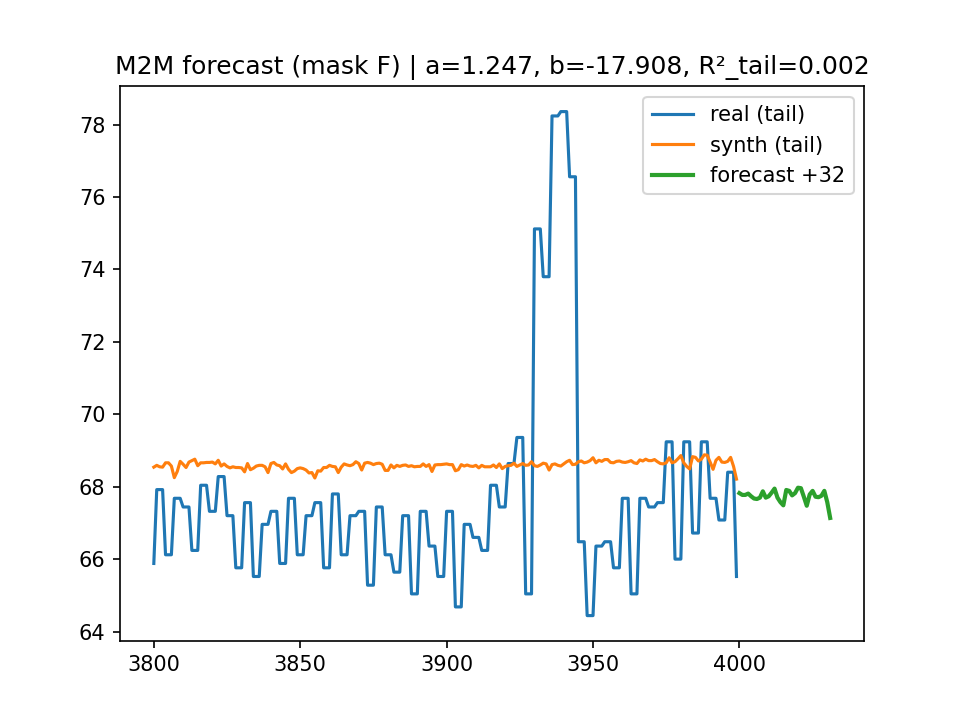
\includegraphics[width=0.78\textwidth]{images/M2M_forecast_32_cal.png}
\caption{Example of forecast on \emph{M2M} ($h{=}32$) with affine calibration on the tail. The green curve represents the predicted values for the following time steps.}
\label{fig:m2m_forecast_cal}
\end{figure}

\subsection{Final observations and considerations}
This experimental analysis showed that \emph{WaveStitch}-based forecasting works effectively when the horizon $h$ remains close to the local dynamics learned within the tail~\cite{wavestitch,tashiro2021csdi}.  
In such cases, as I will show in the next chapter, the \textbf{affine calibration} systematically reduces MAE and RMSE while improving correlation, especially when the bias between real and synthetic data is approximately constant~\cite{bishop2006pattern,box2015time}.  
As $h$ increases, the error tends to be dominated by regime shifts or rare events (peaks, transitions) that cannot be captured from tail information alone~\cite{shumway2017time}.

\medskip
\noindent I also highlight the following operational remarks:
\begin{itemize}
  \item \textbf{Horizon and mask:} the joint choice of $h$ and mask (F/C/M) determines the contextual level. Denser windows (\texttt{F}) are ideal for very short-term forecasts, while coarser ones favor trend stability.
  \item \textbf{Calibration:} the local estimate of $(a,b)$ on the tail (\texttt{tail\_fit}) provides an economical and stable correction; adding ridge regularization helps in the presence of noise.
  \item \textbf{Time alignment:} \emph{future-based} evaluation requires consistent timestamps; a matching tolerance (e.g., \texttt{5min}) helps reduce mismatches and false negatives.
  \item \textbf{Robustness:} future outliers may reduce correlation even with low MAE/RMSE; in such cases, calibration maintains overall scale consistency, while outlier-aware preprocessing can improve pointwise correlation.
\end{itemize}

Therefore, I can conclude that the forecasting module provides \textbf{consistent, calibrated, and controllable} short-term forecasts, achieving a solid compromise between statistical fidelity and numerical stability.  
Finally, in the next chapter, we will examine in detail the quantitative results broken down by dataset, horizon, and mode (raw vs calibrated), which I obtained in this study~\cite{hastie2009elements,shumway2017time,aggarwal2015data}.